%%%%%%%%%%%%%%%%%%%%%%%%%%%%%%%%%%%%%%%%%
% CN2 Labreport template
%
% License:
% CC BY-NC-SA 3.0 (http://creativecommons.org/licenses/by-nc-sa/3.0/)
%
%%%%%%%%%%%%%%%%%%%%%%%%%%%%%%%%%%%%%%%%%

\documentclass[parskip=full]{scrartcl}

\usepackage{siunitx}  % Provides the \SI{}{} command for typesetting SI units
\usepackage{graphicx} % Required for the inclusion of images
\usepackage{booktabs} % nicer tables
\usepackage[noabbrev]{cleveref} % automatic references
\usepackage{listings} % typeset code
\usepackage[backend=biber]{biblatex}
\addbibresource{referenzen.bib}

\crefname{lstlisting}{listing}{listings} % for referencing code
\Crefname{lstlisting}{Listing}{Listings} % for referencing code

\usepackage[headsepline]{scrlayer-scrpage} % header
\ohead{Group 06} % right part of header
\ihead{Assignment 4} % left part of header

\lstset{basicstyle=\ttfamily} % monospaced font in listing



%----------------------------------------------------------------------------------------
%	DOCUMENT INFORMATION
%----------------------------------------------------------------------------------------

\begin{document}
\begin{titlepage}
    \centering
    \vspace*{2cm}
    {\Huge \textbf{Communication Networks 2}}\\
    SS 2021\\
    \vspace*{1cm}
    {\Large Assignment 4}
    \\\vspace*{3cm}
    {\Large \textbf{Group 06}}\\
    \vspace*{1cm}
    {\large 
        \begin{tabular}{l c c}
            Name & Mat.Nummer \\ \hline
            Paul Kloker & 12034928 \\
            Juan Aramis Oposich & 11701238
        \end{tabular}
    }
    \\\vspace*{7cm}
    \today
\end{titlepage}

%----------------------------------------------------------------------------------------
%	SECTION 1
%----------------------------------------------------------------------------------------
\section{Task description} \label{sec:task}

%----------------------------------------------------------------------------------------
%	SECTION 2
%----------------------------------------------------------------------------------------
\section{NS3 Model} \label{sec:procedure}


\begin{verbatim}
$ nmap --privileged -sn -n -T5 --min-parallelism 100 --min-hostgroup 100 
10.0.0.0/16
\end{verbatim}


\begin{table}[hb]
	\centering
	\begin{tabular}{|llll|}
		\hline
		\textbf{No.} & \textbf{Network} & \textbf{IP address} &\textbf{latency}  \\ 
		\hline
		1 & 10.0.0.0/8 & 10.0.4.1 &0.0075s\\
		%\hline
		2 & 10.0.0.0/8 & 10.0.4.2 &0.23s\\
		\hline
		3 & 10.0.0.0/8 & 10.0.120.1 &0.20s\\
		%\hline
		4 & 10.0.0.0/8 & 10.0.120.2 &0.0085s\\
		\hline
		5 & 10.0.0.0/8 & 10.0.132.1 &0.024s\\
		%\hline
		6 & 10.0.0.0/8 & 10.0.132.68 &0.18s\\
		\hline
		7 & 10.0.0.0/8 & 10.0.248.1 &0.78s\\
		%\hline
		8 & 10.0.0.0/8 & 10.0.248.2 &0.16s\\
		\hline
		\hline
		9 & 10.1.0.0/8 & 10.1.6.1 &0.18s\\
		%\hline
		10 & 10.1.0.0/8 & 10.1.6.110 &0.18s\\
		\hline
		11 & 10.1.0.0/8 & 10.1.7.1 &1.5s\\
		%\hline
		12 & 10.1.0.0/8 & 10.1.7.123 &0.78s\\
		\hline
	\end{tabular}
	\caption{Discovered IP addresses}
	\label{tab:nmap}
\end{table}

\section{Data analysis and comparison} \label{sec:data}


\begin{table}[hb]
	\centering
	\begin{tabular}{ll}
		\toprule
		\textbf{End-to-End delay} & \textbf{User experience} \\ \midrule
			$T_{EE} < 150$ & acceptable for all users \\
			$150 < T_{EE} < 300$ & noticeable quality degradation, but still acceptable for most users\\
			$T_{EE} \geq 300$ & not acceptable\\
			\bottomrule
		\end{tabular}
		\caption{Delay to user experience}
		\label{tab:delayEnd2End}
	\end{table}

\begin{figure}[!ht]
	\centering % centering figure 
	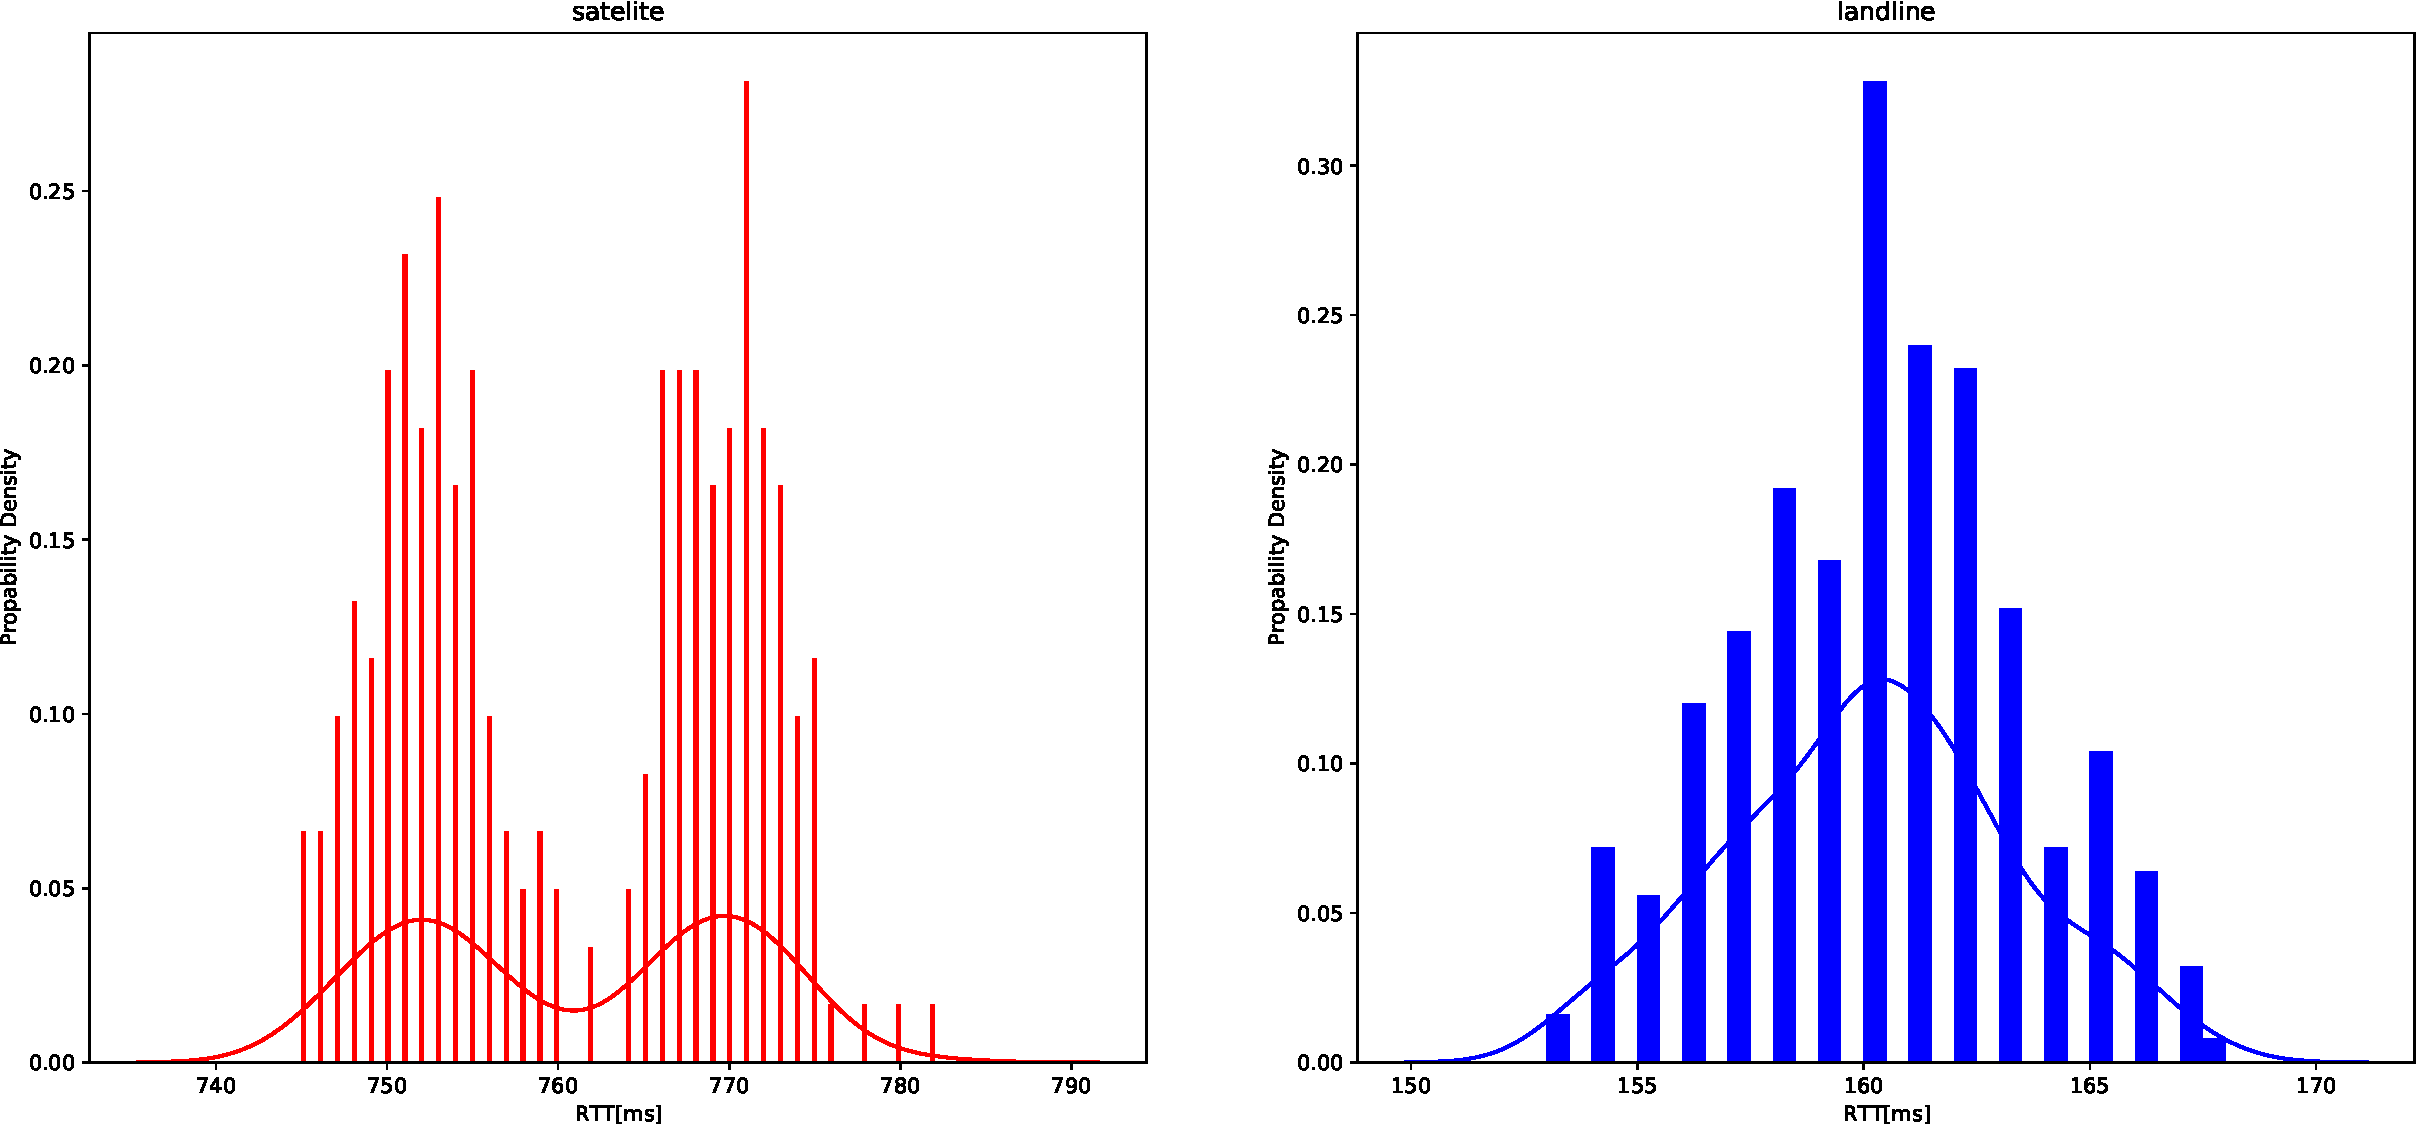
\includegraphics[width=\textwidth]{images/oneWayDelay.pdf} % importing figure
	\caption{Propobility density of one way delay} 
	\label{fig:one-way-delay} % labeling to refer it inside the text
\end{figure}


%----------------------------------------------------------------------------------------
%	SECTION 3
%----------------------------------------------------------------------------------------

\section{Conclusion}



%----------------------------------------------------------------------------------------
%	SECTION X
%---------------------------------------------------------------------------------------

\printbibliography

\end{document}
